\subsection{Griewank 1D}

\par The Griewank function is a function that is typically used for testing optimization. The function is defined by:

$$
f_1(x) = 1+(1/4000)\cdot x_1^2-\cos(x_1)
$$

It has multiple maxima and minima but its global minima is at $x=0$.

\par Both functions are tested five times with the Griewank function with the same starting random population and a dimensional space of [-100, 100].

\begin{table}[ht]
\scriptsize
\begin{tabular}{l|ccccc}
\textbf{}        & \textbf{Trial 1} & \textbf{Trial 2} & \textbf{Trial 3} & \textbf{Trial 4} & \textbf{Trial 5} \\
\hline
LOA End Fitness  & 1.5846E-07       & 1.2658E-07       & 7.4251E-08       & 3.5575E-06       & 5.4992E-08       \\
LOA Evaluations  & 3499             & 3453             & 3465             & 3560             & 3468             \\
iLOA End Fitness & 9.3769E-10       & 3.1541E-13       & 4.5715E-11       & 1.8532E-09       & 2.1836E-12       \\
iLOA Evaluations & 3042             & 2803             & 2710             & 2718             & 2857
\end{tabular}
\caption{ \scriptsize LOA vs. iLOA: Griewank 1D ($f_1$)}
\end{table}

\begin{figure}
  \centering
  \begin{subfigure}[b]{0.4\textwidth}
    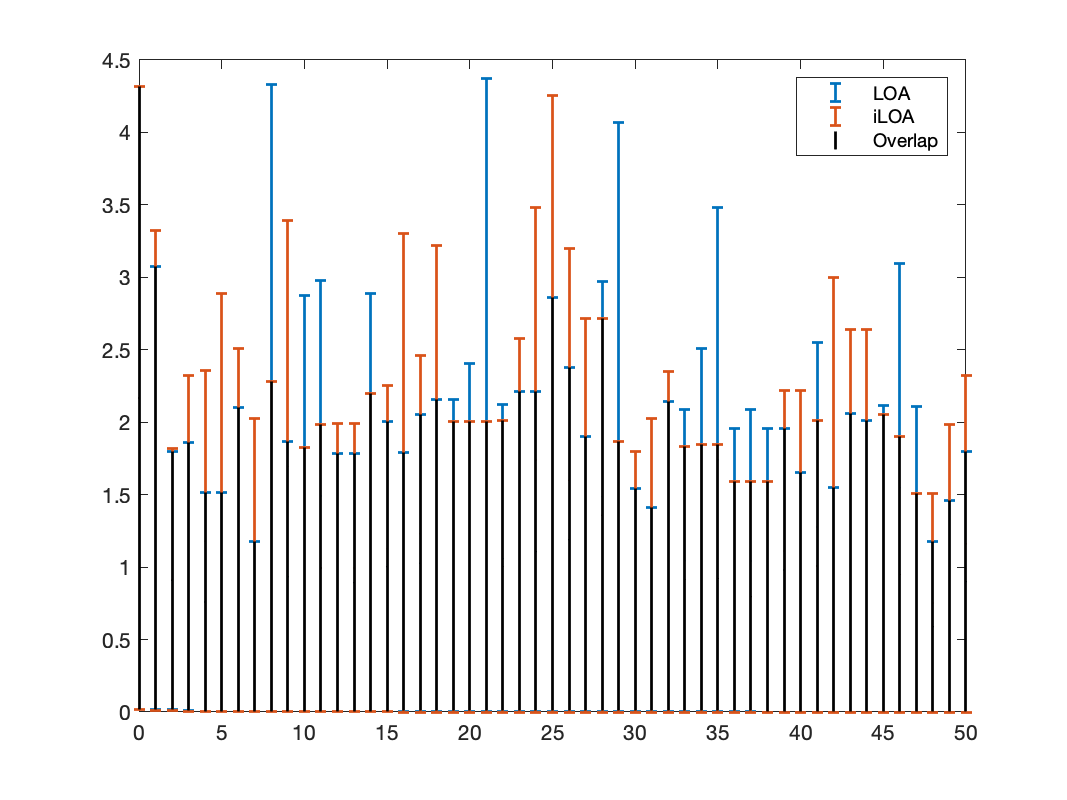
\includegraphics[width=\textwidth]{img/bars/f1/1}
    \caption{ \scriptsize Trial 1: Fitness Range (y) over Iterations (x)}
    \label{fig:f1-b-1}
  \end{subfigure}
  \begin{subfigure}[b]{0.4\textwidth}
    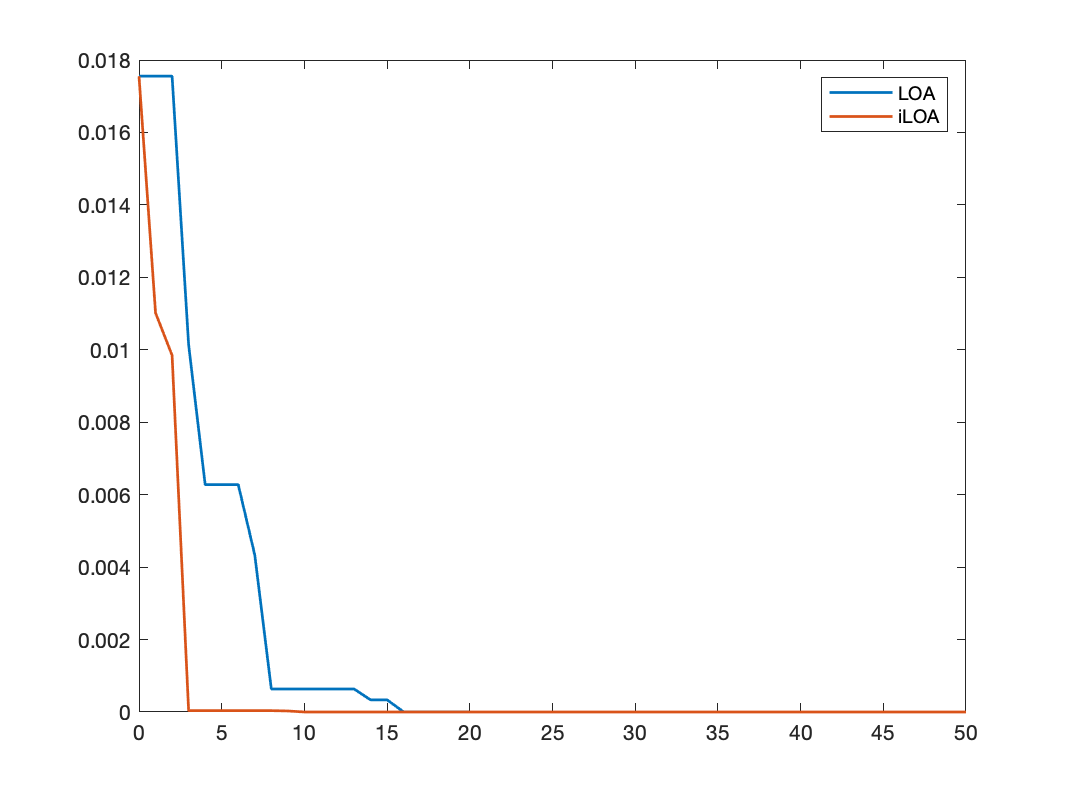
\includegraphics[width=\textwidth]{img/fits/f1/1}
    \caption{ \scriptsize Trial 1: Minimum Fitness (y) over Iterations (x)}
    \label{fig:f1-f-1}
  \end{subfigure}

  \begin{subfigure}[b]{0.4\textwidth}
    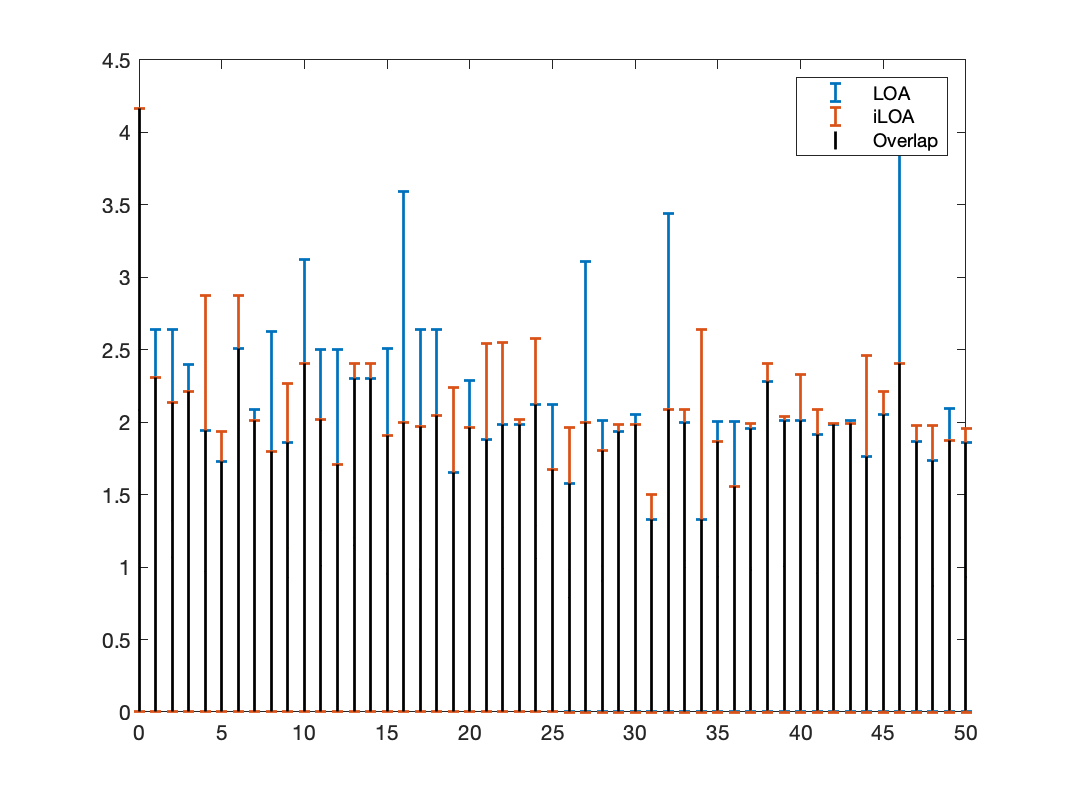
\includegraphics[width=\textwidth]{img/bars/f1/2}
    \caption{ \scriptsize Trial 2: Fitness Range (y) over Iterations (x)}
    \label{fig:f1-b-2}
  \end{subfigure}
  \begin{subfigure}[b]{0.4\textwidth}
    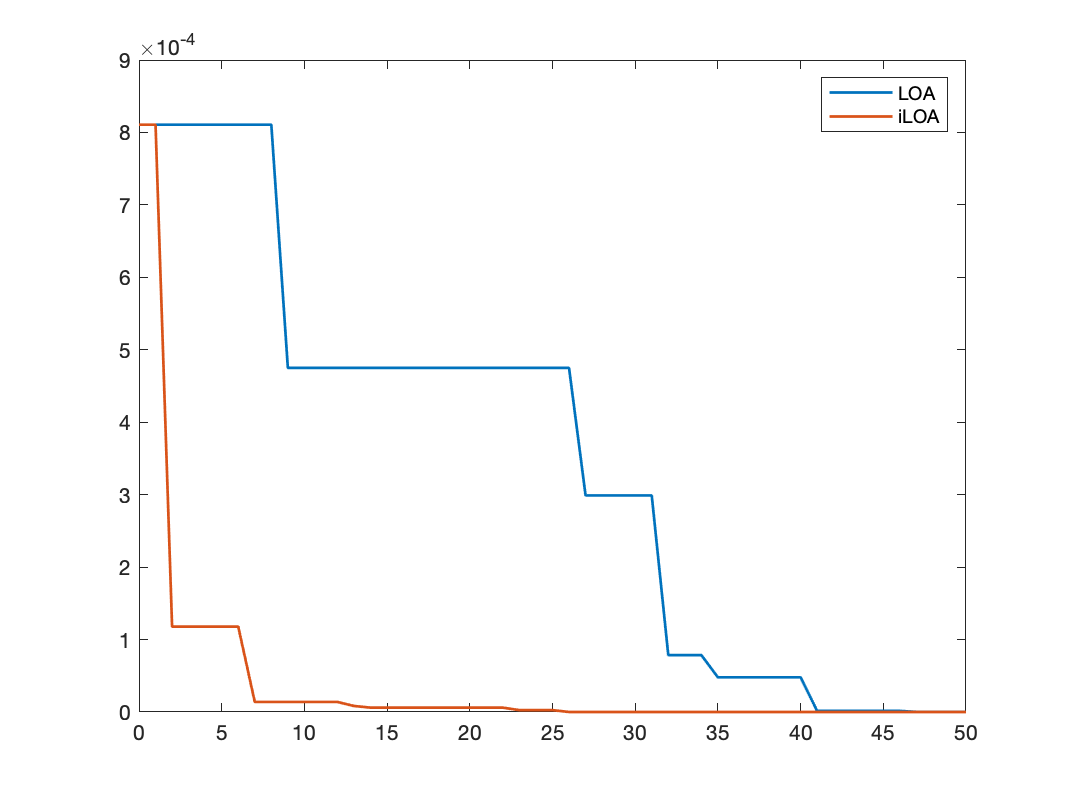
\includegraphics[width=\textwidth]{img/fits/f1/2}
    \caption{ \scriptsize Trial 2: Minimum Fitness (y) over Iterations (x)}
    \label{fig:f1-f-2}
  \end{subfigure}

  \begin{subfigure}[b]{0.4\textwidth}
    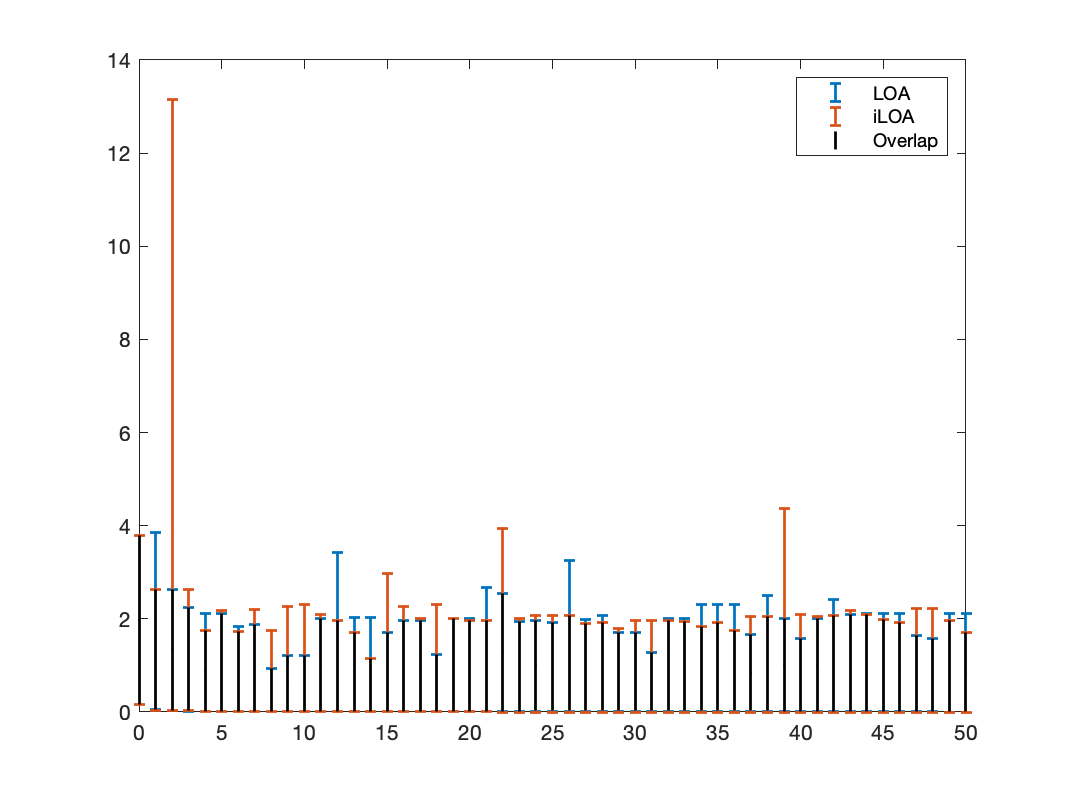
\includegraphics[width=\textwidth]{img/bars/f1/3}
    \caption{ \scriptsize Trial 3: Fitness Range (y) over Iterations (x)}
    \label{fig:f1-b-3}
  \end{subfigure}
  \begin{subfigure}[b]{0.4\textwidth}
    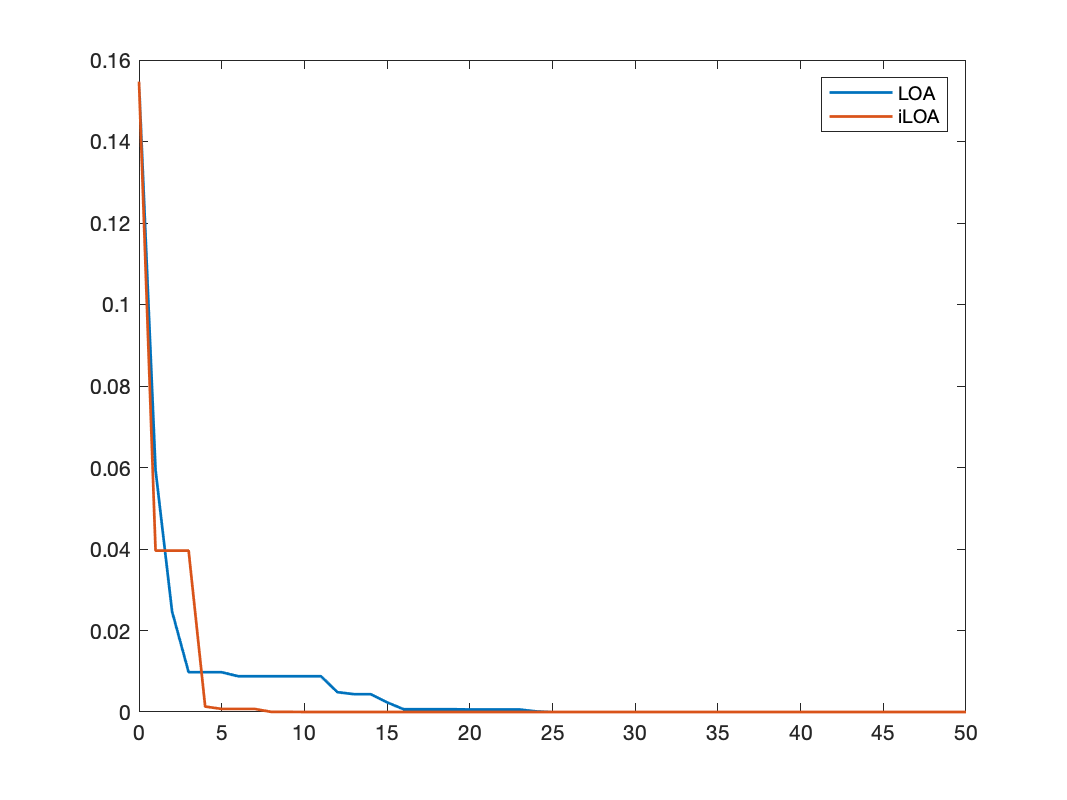
\includegraphics[width=\textwidth]{img/fits/f1/3}
    \caption{ \scriptsize Trial 3: Minimum Fitness (y) over Iterations (x)}
    \label{fig:f1-f-3}
  \end{subfigure}

  \begin{subfigure}[b]{0.4\textwidth}
    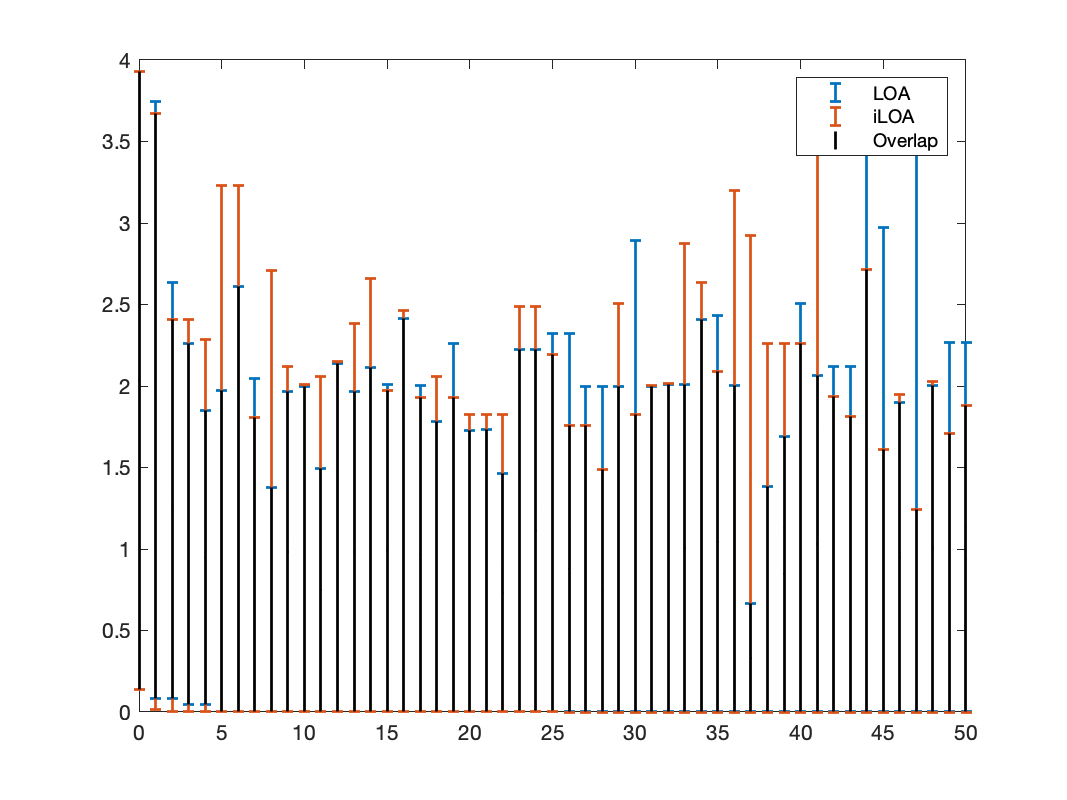
\includegraphics[width=\textwidth]{img/bars/f1/4}
    \caption{ \scriptsize Trial 4: Fitness Range (y) over Iterations (x)}
    \label{fig:f1-b-4}
  \end{subfigure}
  \begin{subfigure}[b]{0.4\textwidth}
    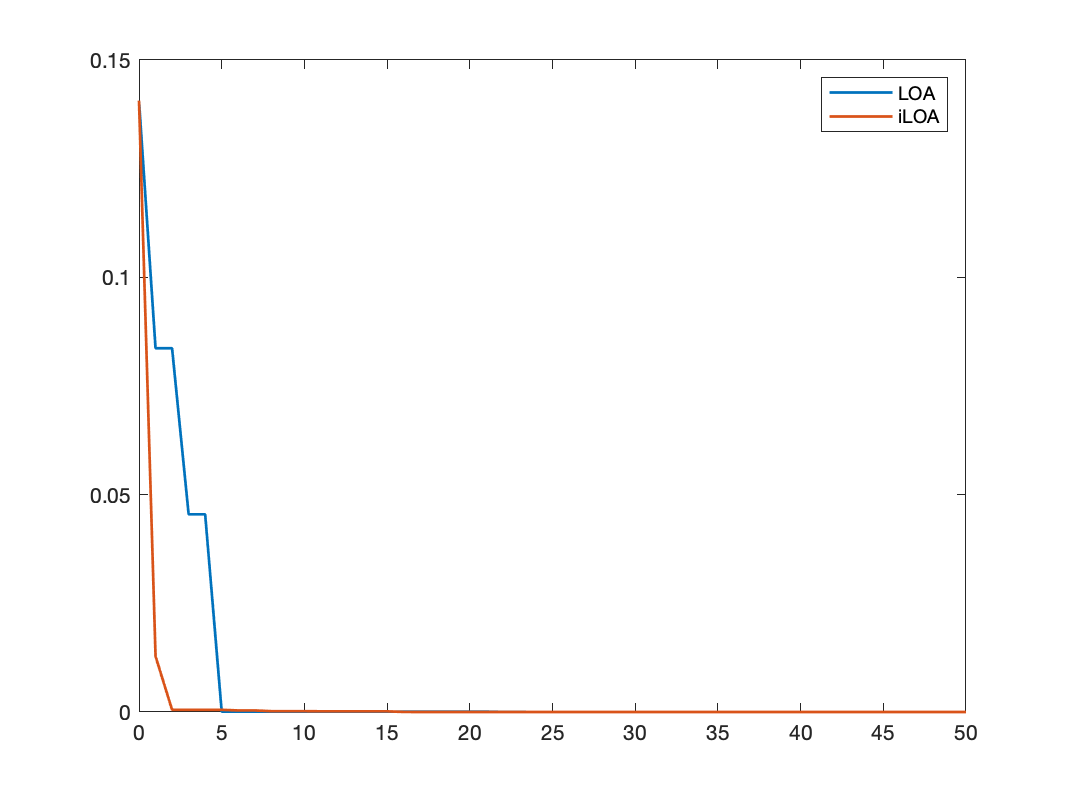
\includegraphics[width=\textwidth]{img/fits/f1/4}
    \caption{ \scriptsize Trial 4: Minimum Fitness (y) over Iterations (x)}
    \label{fig:f1-f-4}
  \end{subfigure}

  \begin{subfigure}[b]{0.4\textwidth}
    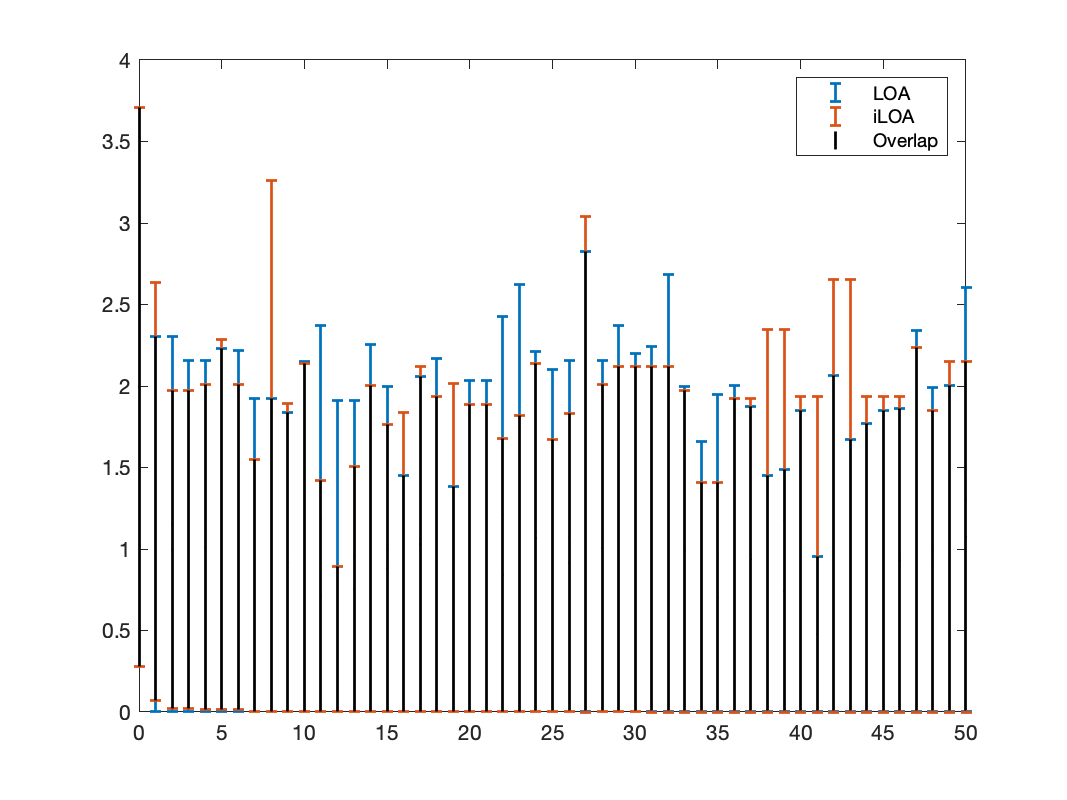
\includegraphics[width=\textwidth]{img/bars/f1/5}
    \caption{ \scriptsize Trial 5: Fitness Range (y) over Iterations (x)}
    \label{fig:f1-b-5}
  \end{subfigure}
  \begin{subfigure}[b]{0.4\textwidth}
    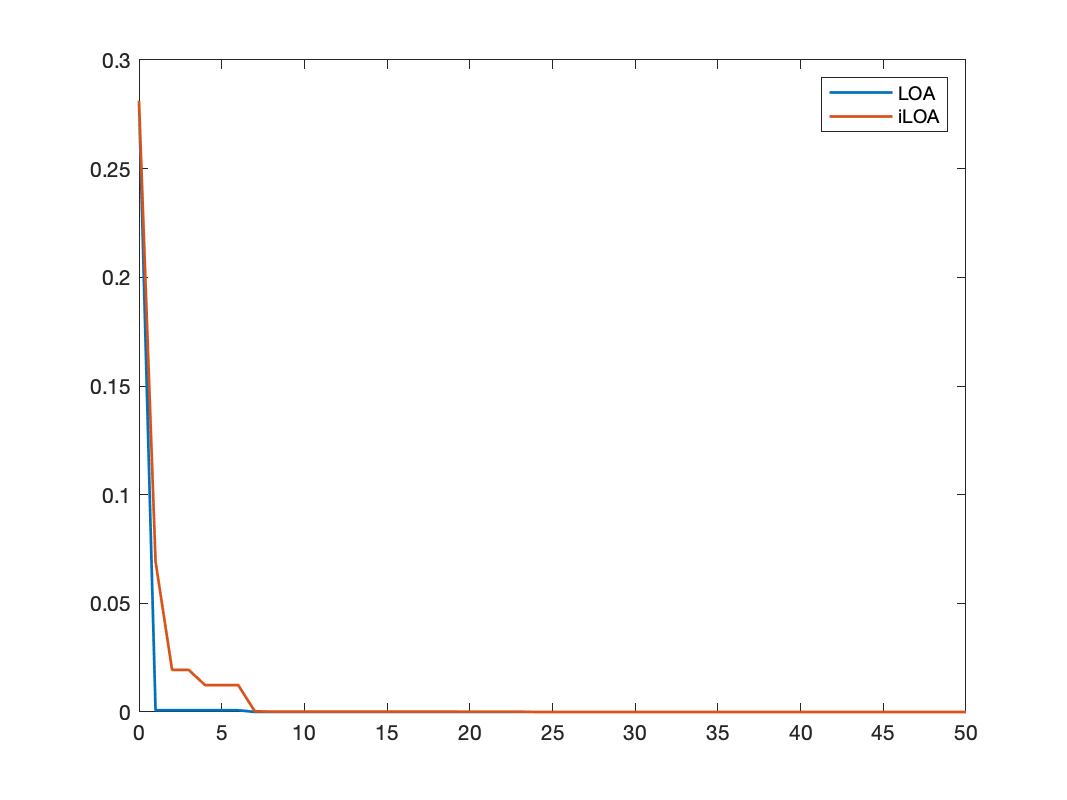
\includegraphics[width=\textwidth]{img/fits/f1/5}
    \caption{ \scriptsize Trial 5: Minimum Fitness (y) over Iterations (x)}
    \label{fig:f1-f-5}
  \end{subfigure}

  \caption{ \scriptsize LOA vs. iLOA: Griewank 1D ($f_1$)}
\end{figure}
